\documentclass[10pt]{article}
\usepackage[a4paper, left=1.5cm, right=1.5cm, top=3.5cm]{geometry}
\usepackage[ngerman]{babel}
\usepackage[]{graphicx}
\usepackage{multicol}
\usepackage{amssymb}
\usepackage{inputenc}
\usepackage{breqn}
\usepackage{titlesec}
\usepackage{wrapfig}
\usepackage{blindtext}
\usepackage{lipsum}
\usepackage{caption}
\usepackage{listings}
\usepackage{fancyhdr}
\usepackage{nopageno}
\usepackage{authblk}
\usepackage{amsmath}
\usepackage{mathtools}
\usepackage{bm}
\usepackage[ISO]{diffcoeff}
\usepackage{xcolor}
\usepackage{csquotes}
\usepackage{siunitx}
\usepackage{circuitikz}
\fancyhf[]{}

\newenvironment{Figure}
  {\par\medskip\noindent\minipage{\linewidth}}
  {\endminipage\par\medskip}

\begin{titlepage}
    \title{Elektronikpraktikum -- Versuch 7: Logische Schaltungen}
    \author[1]{Jonas Wortmann\thanks{s02jwort@uni-bonn.de}}
    \author[1]{Angelo V. Brade\thanks{s72abrad@uni-bonn.de}}
    \affil[1]{Rheinische Friedrich-Wilhelms-Universität Bonn}
    \date{\today}
\end{titlepage}

\begin{document}
\pagenumbering{gobble}
\maketitle
\newpage

\tableofcontents
\newpage

\pagenumbering{arabic}

\pagestyle{fancy}
\fancyhead[R]{\thepage}
\fancyhead[L]{\leftmark}


\begin{multicols}{2}
	\section{Einleitung}
  Dieser Versuch ist die Einführung in die boolische Elektrotechnik, wobei wir boolische Algebra nutzen, um logische Operationen zu konstruieren und z.B. Flip-Flops bauen, mit denen wir ein Shreiberegister und Zähler bauen. Dabei basiert alles darauf, dass hohe Spannungen einer logsichen 1 zugeordnet werden und niedrige Spannungen einer logischen 0 zugeordnet werden. Von hier aus wird die grundlegende Informatik praktisch aufgebaut.

	\section{Theorie}
	\subsection{Boolische Algebra und Schaltfunktionen}
	Bei digitalen Schalftelementen gibt es im allgmeinen mehrere Eingänge und einen Ausgang, wobei alle Signal als 0 oder 1 interpretiert werden. Das Verhalten lässt sich mit Schaltfunktionen beschreiben, die von der Menge der Eingangsvariablen auf die Menge der Ausgangsvariable abbildet. Um diese Funktionen darzustellen werden Funktionstafeln verwendet, die alle Kombinationen an Eingängen, sowie die zugeordneten Ausgang angeben.

	Für eine Eingangsvariable sind die folgenden operationen möglich:
	\begin{align*}
		 & \textbf{Identität}                                  & p(x) = x       \\
		 & \textbf{Komplement} \text{ oder } \textbf{Negation} & p(x) = \bar{x} \\
		 & \text{sowie konstant 1}                             & p(x) = 0       \\
		 & \text{und konstant 0}                               & p(x) = 1
	\end{align*}

	Für Funktionen mit zwei Eingansvariablen, sog. elementare Funktionen, sind diese möglich:
	\begin{center}
		\begin{tabular}{|c|c|c|c|}
			\hline
			      &       & \textbf{Konjunktion} & \textbf{Disjunktion} \\
			$x_1$ & $x_2$ & \textbf{UND}         & \textbf{ODER}        \\
			      &       & $x_1 \cdot x_2$      & $x_1 + x_2$          \\
			\hline
			0     & 0     & 0                    & 0                    \\
			0     & 1     & 0                    & 1                    \\
			1     & 0     & 0                    & 1                    \\
			1     & 1     & 1                    & 1                    \\
			\hline
		\end{tabular}
		\captionof{table}{Elementare Funktionen}
	\end{center}

	Nun lässt sich jede boolesche Funktion F als Summe von Mintermen, die sog. disjunktive Normalform, oder als Produkt von Maxtermen, die sog. konjunktive Normalform, ausdrücken. Hierbei ist eine Minterm $m$ eine boolesches Produkt aus jeder Eingangsvariable oder ihrem Kompliment, wobei diese jeweils nur einmal auftreten. Genauso ist ein Maxterm $M$ eine boolesche Summer aus jeder Eingangsvariable oder ihrem Kompliment, wobei diese jeweils nur einmal auftreten.
	Hier sind gebräuchliche Schalftunktionen dargestellt:
	\begin{Figure}
		\centering
		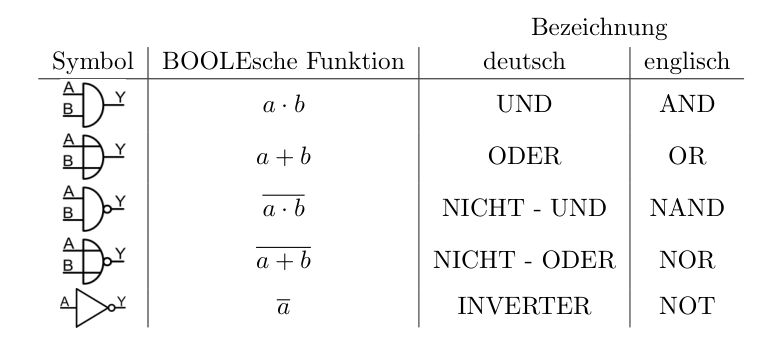
\includegraphics[width=1\textwidth]{schaltfunktionen.png}
		\captionof{figure}{Gebräuchliche Schaltfunktionen}
	\end{Figure}
	\subsection{Flip-Flops}
	Die einfachste möglichkeit ein Signal zu speicher, ist mithilfe eines Flip-Flops.
	\begin{Figure}
		\centering
		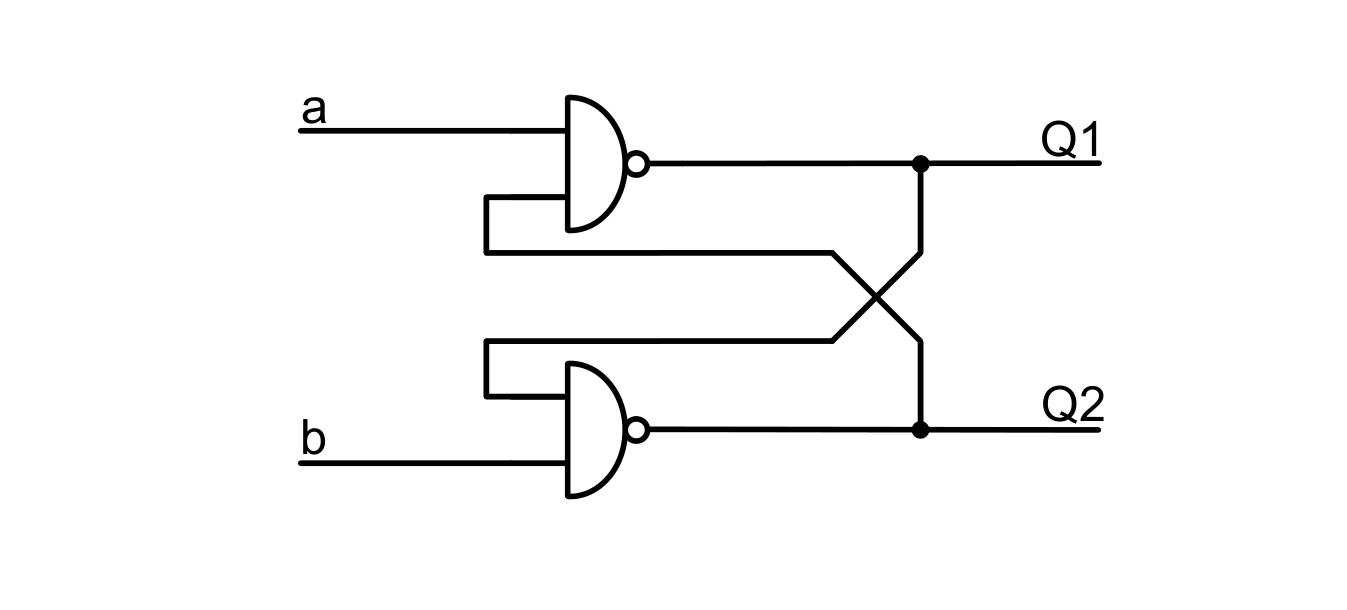
\includegraphics[width=1\textwidth]{fliflop.png}
		\captionof{figure}{Flip-Flop}
	\end{Figure}
	Ist $a=b=1$, so ist das signal gespeichert und es lässt sich durch belegen mit einer 0 löschen. Hierbei ist dann $Q_2=\overline{Q_1}$ gespeichert.
	\subsection{Schrieberegister und Zähler}
	Nun kann man mithilfe von FFs eine Schreibregister bauen, dass mit jedem Takt den Inhalt des $i$-ten FFs in das $(i+1)$-te FF schreibt. Neben dem gibt es dann noch den Dualzähler. Er erzeugt in ansteigender Reinfolge mit jedem Takt Dualzahlen.
	\subsection{Aufbau von elektronischen Logikschaltungen}
	Um nun Logikschaltungen zu konstruieren, wird eine Minimalspannung, ab der das Signal als 1 interpretiert wird, und eine Maximalspannung, unter der das Signal als 0 interpretiert wird, definiert. Diese Schwellspannungen lassen sich in Übertragungskennlinien darstellen, hier in Abb. \ref{fig:kennlinie}.
	\begin{Figure}
		\centering
		\includegraphics[width=1\textwidth]{übetragungskennlinie.png}
		\captionof{figure}{Übertragungskennlinie eines Inverters}
		\label{fig:kennlinie}
	\end{Figure}
	\begin{Figure}
		\centering
		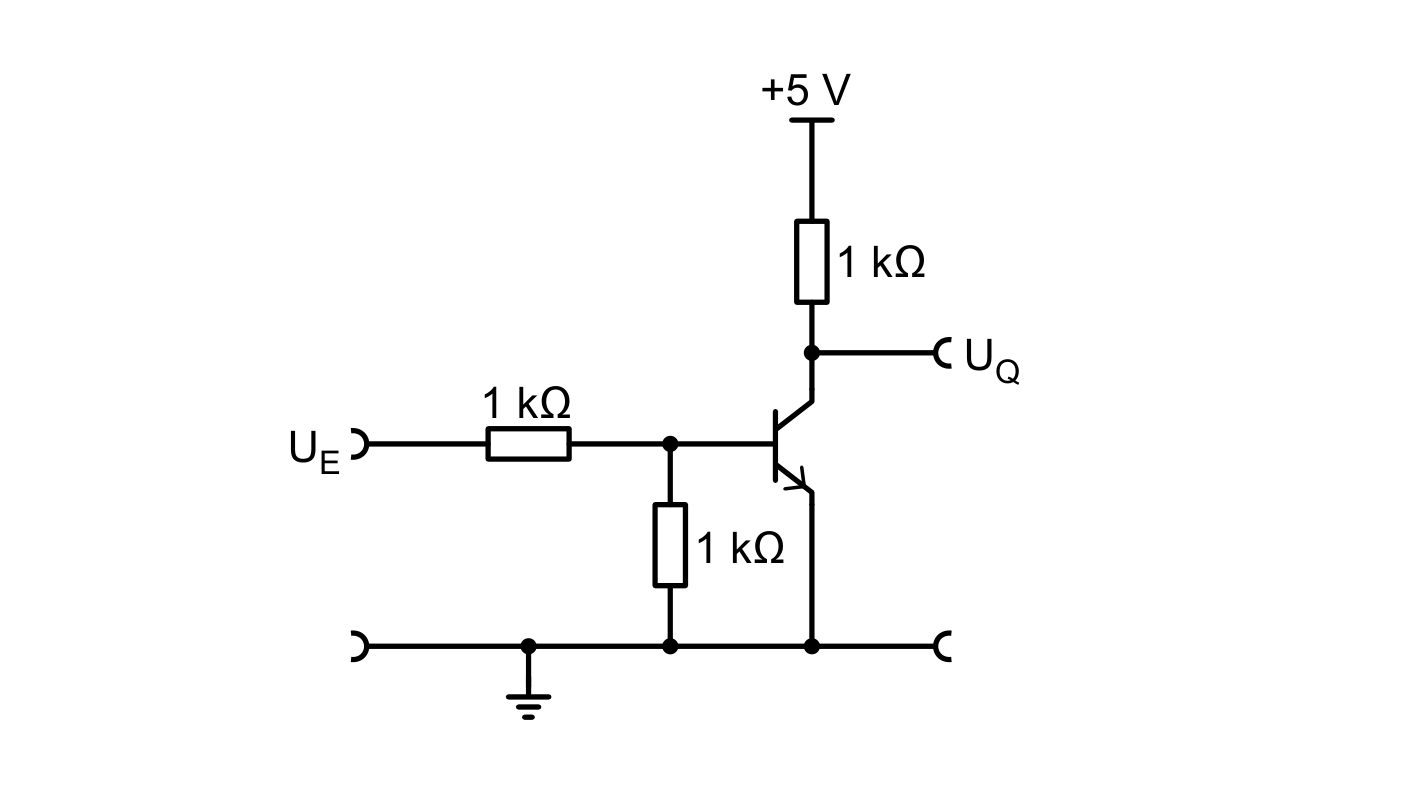
\includegraphics[width=1\textwidth]{inverter.png}
		\captionof{figure}{Schaltung eines Inverters}
		\label{fig:inverter}
	\end{Figure}
	Z.B ein Inverter kann nun mit Transistoren realisiert werden. Hier in Abb. \ref{fig:inverter} dargestellt. Diese Schaltung kann mit z.B. Dioden erweitert werden, um mehr Eingänge zu erhalten. Dies wird allerding heutzutage nicht mehr mit Diodon, sondern direkt mit Transistoren gemacht, da diese deutlich kleiner hergestellt werden können. So kann auch ein CMOS-Gatter realisiert werden, welches allein aus Transistoren besteht und somit extrem klein gebaut werden kann. Dies ist hier in Abb. \ref{fig:gatter} dargestellt.
	\begin{Figure}
		\centering
		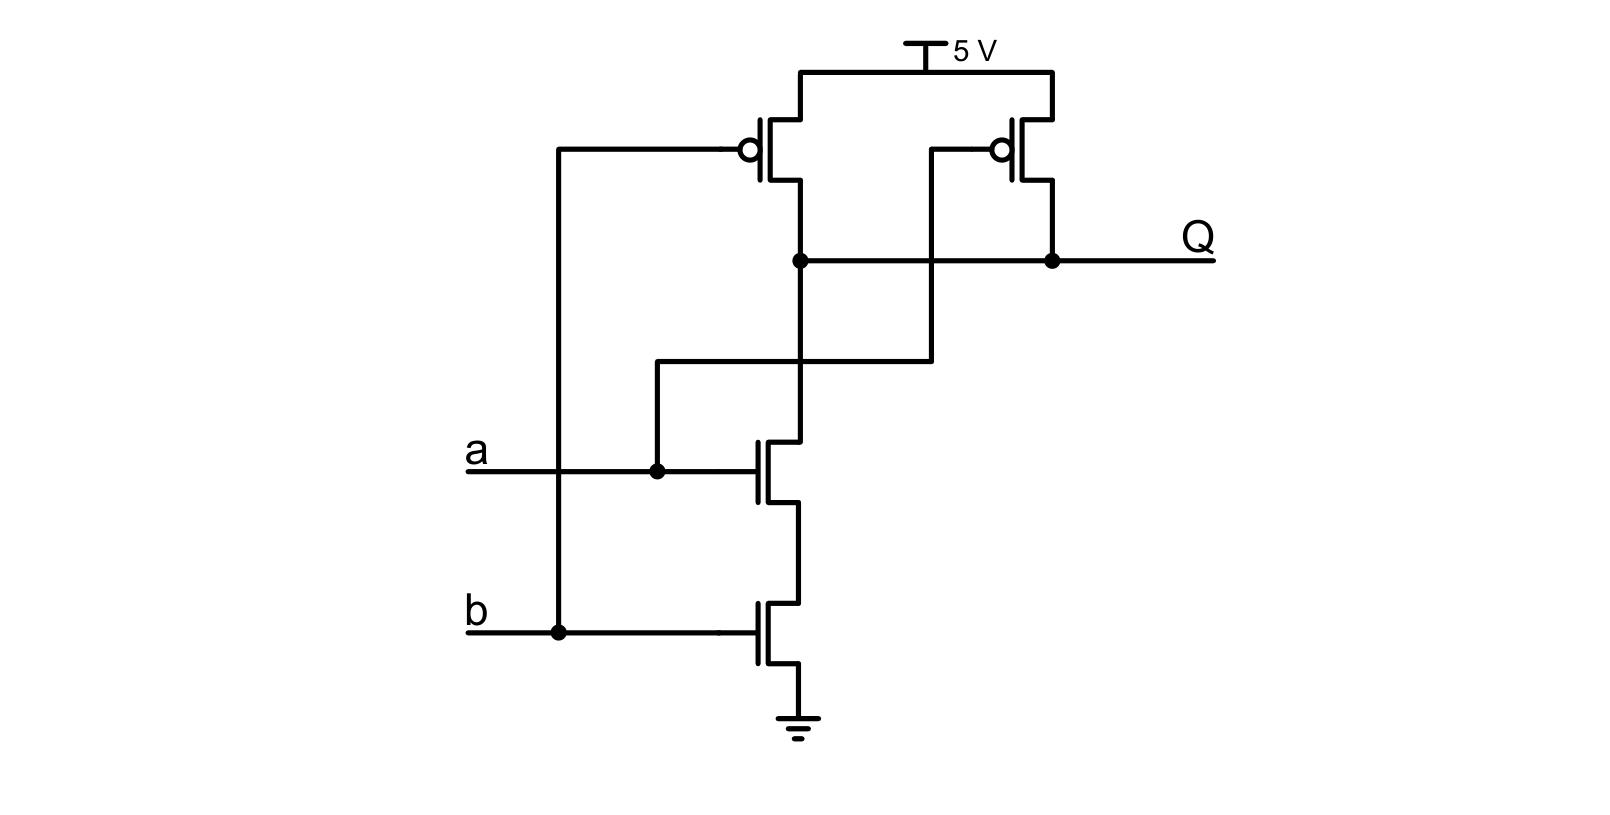
\includegraphics[width=1\textwidth]{cmos-gatter.png}
		\captionof{figure}{Schaltung eines CMOS-Gatter}
		\label{fig:gatter}
	\end{Figure}
	\section{Voraufgaben}
	\subsection*{A}
	Wenn man $n$ Eingangsvariablen hat, gibt es ohne Redundanzen $2^{2n}$ Schaltfunktionen.
	\subsection*{B}
	Es werden folgende Ausdrücke mit einer Funktionstafel überprüft.
	\begin{align*}
		a + 1 & = 1 \quad & a \cdot 1 & = a \quad & a + \bar{a}     & = 1 \\
		a + 0 & = a \quad & a \cdot 0 & = 0 \quad & a \cdot \bar{a} & = 0
	\end{align*}
	Man erkennt in Tab. \ref{tab:ftafel}, dass alle Ausrücke korrekt sind.

	\begin{center}
		\begin{tabular}{|c|c|c|c|}
			\hline
			\textbf{Funktion $f$} & $a$ & $\bar{a}$ & $f(a, \bar{a})$ \\
			\hline
			$a + 1$               & 0   & 1         & 1               \\
			                      & 1   & 0         & 1               \\
			\hline
			$a + 0$               & 0   & 1         & 0               \\
			                      & 1   & 0         & 1               \\
			\hline
			$a \cdot 1$           & 0   & 1         & 0               \\
			                      & 1   & 0         & 1               \\
			\hline
			$a \cdot 0$           & 0   & 1         & 0               \\
			                      & 1   & 0         & 0               \\
			\hline
			$a + \bar{a}$         & 0   & 1         & 1               \\
			                      & 1   & 0         & 1               \\
			\hline
			$a \cdot \bar{a}$     & 0   & 1         & 0               \\
			                      & 1   & 0         & 0               \\
			\hline
		\end{tabular}
		\captionof{table}{Funktionstafel}
		\label{tab:ftafel}
	\end{center}
	\subsection*{C}
	Nun wird das Distributivgesetz und das Gesetz von DeMorgan mithilfe von Funktionstafeln bestätigt. Diese sind in Tab. \ref{tab:dis} und \ref{tab:morg} dargestellt.
	\begin{center}
		\begin{tabular}{|c|c|c|c|c|c|c|c|c|}
			\hline
			$a$ & $b$ & $c$ & $a + b$ & $(a + b) \cdot c$ & $a \cdot c$ & $b \cdot c$ & $a \cdot c + b \cdot c$ \\
			\hline
			0   & 0   & 0   & 0       & 0                 & 0           & 0           & 0                       \\
			0   & 0   & 1   & 0       & 0                 & 0           & 0           & 0                       \\
			0   & 1   & 0   & 1       & 0                 & 0           & 0           & 0                       \\
			0   & 1   & 1   & 1       & 1                 & 0           & 1           & 1                       \\
			1   & 0   & 0   & 1       & 0                 & 0           & 0           & 0                       \\
			1   & 0   & 1   & 1       & 1                 & 1           & 0           & 1                       \\
			1   & 1   & 0   & 1       & 0                 & 0           & 0           & 0                       \\
			1   & 1   & 1   & 1       & 1                 & 1           & 1           & 1                       \\
			\hline
		\end{tabular}

		\captionof{table}{Funktionstafel für das Distributivgesetz}
		\label{tab:dis}
	\end{center}
	\begin{center}
		\begin{tabular}{|c|c|c|c|c|c|c|c|c|c|c|}
			\hline
			$a$ & $b$ & $\bar{a}$ & $\bar{b}$ & $a \cdot b$ & $\overline{a\cdot b}$ & $\bar{a} + \bar{b}$ & $a + b$ & $\bar{a + b}$ & $\overline{a} \cdot \bar{b}$ \\
			\hline
			0   & 0   & 1         & 1         & 0           & 0                     & 1                   & 0       & 1             & 1                            \\
			0   & 1   & 1         & 0         & 0           & 1                     & 0                   & 1       & 0             & 1                            \\
			1   & 0   & 0         & 1         & 0           & 0                     & 1                   & 1       & 1             & 0                            \\
			1   & 1   & 0         & 0         & 1           & 0                     & 0                   & 1       & 0             & 0                            \\
			\hline
		\end{tabular}
		\captionof{table}{Funktionstafel für das DeMorgan-Gesetz}
		\label{tab:morg}
	\end{center}
	\subsection*{D}
	\begin{align}
		f(a, b) & = (a + b) \cdot (\overline{a\cdot b})
		        & =
	\end{align}
	Der ausruck folgt der Tabelle, allerdings beschriebt $\overline{(a\cdot b)}$ nicht die Tabelle.
	\subsection*{E}
	Da wir für jede Variable entweder die normale Form oder die negierte Form und somit zwei Zustände haben, und wir jede Kombination durchgehen wollen, kann man binär hochzählen, wobei dann 0 für normal und 1 für negiert steht.
	\begin{center}
		\begin{tabular}{|c|c|}
			\hline
			Binäre Zahl & entsprechender Minterm                               \\
			\hline
			000         & $a \cdot b \cdot c$                                  \\
			001         & $a \cdot b \cdot \overline{c}$                       \\
			010         & $a \cdot \overline{b} \cdot c$                       \\
			011         & $a \cdot \overline{b} \cdot \overline{c}$            \\
			100         & $\overline{a} \cdot b \cdot c$                       \\
			101         & $\overline{a} \cdot b \cdot \overline{c}$            \\
			110         & $\overline{a} \cdot \overline{b} \cdot c$            \\
			111         & $\overline{a} \cdot \overline{b} \cdot \overline{c}$ \\
			\hline
		\end{tabular}
		\captionof{table}{Mintermbestimmung mithilfe von binärem Zählen.}
	\end{center}
	\subsection*{F}
	Sobald $a$ und $b$, 1 sind, sind die Ausgänge nicht mehr eindeutig. Für sonnstige Zustände sind die Ausgänge eindeutig.
	\begin{center}
		\begin{tabular}{|c|c|c|c|}
			\hline
			$a$ & $b$ & $Q_1$    & $Q_2$    \\
			\hline
			0   & 0   & 1        & 1        \\
			0   & 1   & 1        & 0        \\
			1   & 0   & 0        & 1        \\
			1   & 1   & 0 oder 1 & 0 oder 1 \\
			\hline
		\end{tabular}
		\captionof{table}{Funktionstafel von einem Flip Flop}
		\label{tab:fff}
	\end{center}
	\subsection*{G}
	Um einen 4-Bit-Schreibergeister zu konstruieren, müssen vier D-FF hinteinander geschalten werden, welche snychron getrakted werden. Dieser ist in Abb. \ref{fig:schreibregister} dargestellt.
	\begin{Figure}
		\centering
		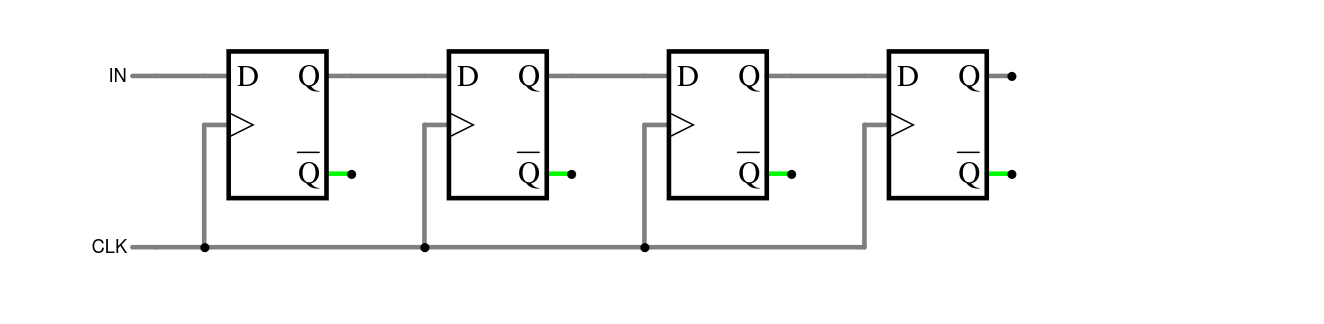
\includegraphics[width=1\textwidth]{circuit-20240908-2016.png}
		\captionof{figure}{4-Bit Schreibregister}
		\label{fig:schreibregister}
	\end{Figure}
	\subsection*{H}
	Ein paralleles Schieberegister wird nach Abb. \ref{fig:paraschreibregister} konstruiert.
	\begin{Figure}
		\centering
		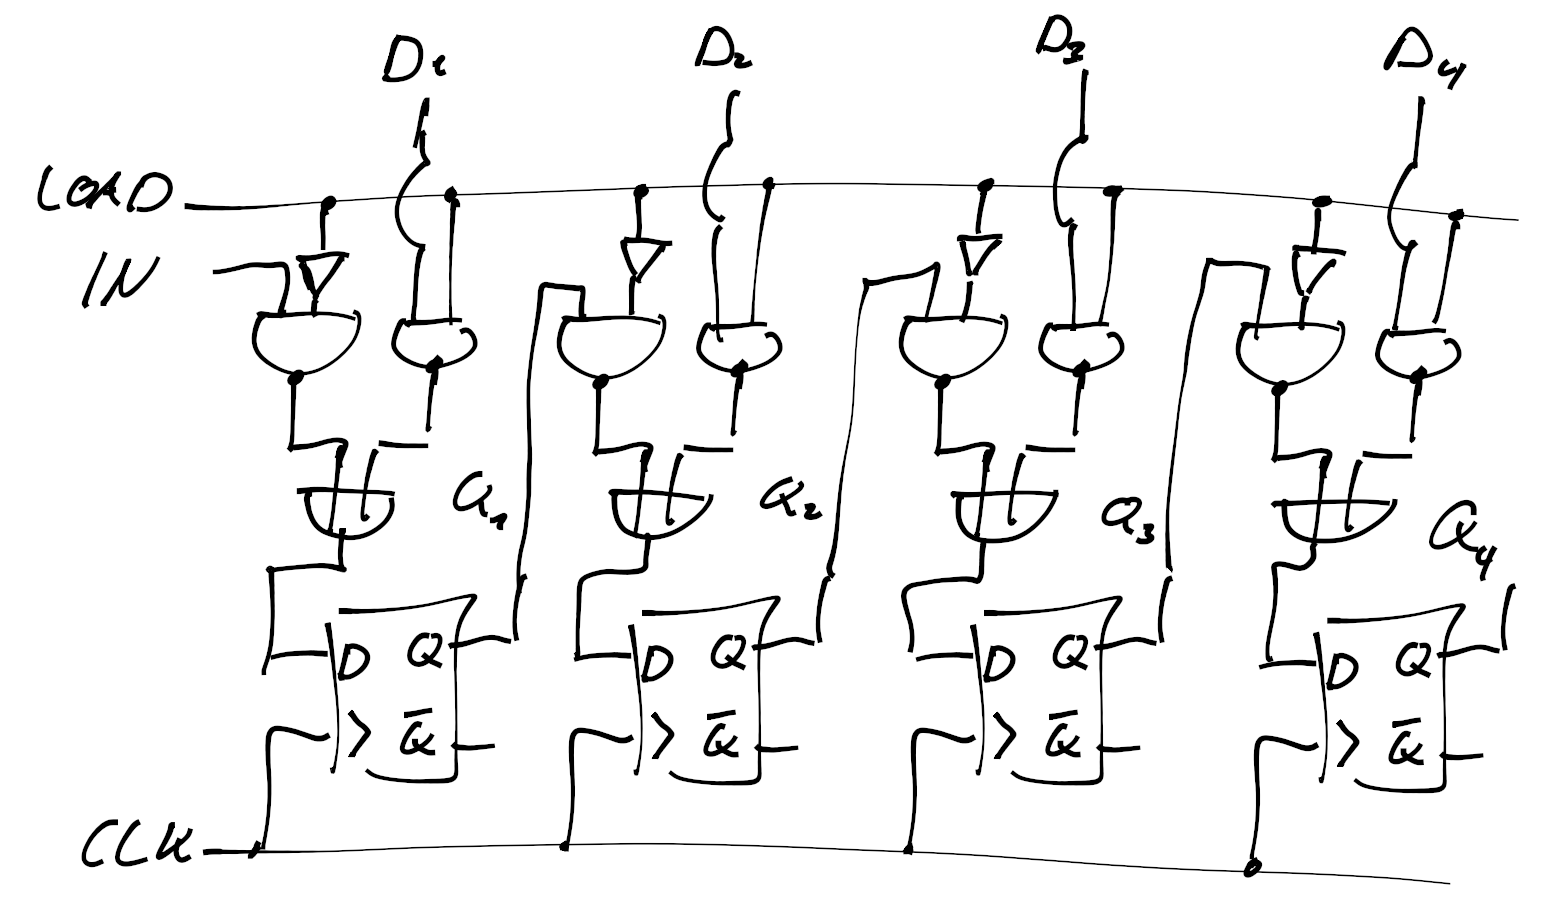
\includegraphics[width=1\textwidth]{parallel-schieberegister.png}
		\captionof{figure}{parallel 4-Bit Schreibregister}
		\label{fig:paraschreibregister}
	\end{Figure}
	\subsection*{I}
	Ein Dualzähler wird nach Abb. \ref{fig:dualzähler} konstruiert.
	\begin{Figure}
		\centering
		\includegraphics[width=1\textwidth]{4bit_dualzähler.png}
		\captionof{figure}{parallel 4-Bit Dualzähler}
		\label{fig:dualzähler}
	\end{Figure}
	\subsection*{J}
	Die Funktion der Schaltung entspricht einer NOR-Schaltung. Die beiden Dioden dienen als Eingangssignal, das aktiviert ist, sobald einer der beiden Eingänge aktiv ist. Somit erhälten wir eine OR-Schaltung. Nun ist hinter den Dioden ein Invertierer geschaltet, welcher das Signal invertiert und so die Schaltung zu einer NOR-Schaltung vervollständigt.

	Da wir eine Basis-Spannung von ca. \SI{1.8}{V} haben und über Basis-Emitter $U_{BE}=\SI{0.7}{V}$ abfällt können wir mit
	\begin{align}
		I_B & =\frac{\SI{1.8}{V}-\SI{0.7}{V}}{\SI{1}{\kilo\Omega}}-\frac{\SI{0.7}{V}}{\SI{1}{\kilo\Omega}} \\
		    & =\SI{0.4}{\milli A}
	\end{align}
	zeigen, dass der Ausgangspegel korrekt ist.
	\subsection*{K}
	Es fließt Strom, aber es gibt probleme.

	Muss noch gemacht werden!!!!!!1
	\subsection*{L}
	Beim CMOS-Inverter fließt bei geringer anliegender Spannung Strom, sodass beim Ausgang Spannung anliegt. Bei hoher Spanung fließt kein Strom, sodass keine Ausgangsspannung anliegt.
	\subsection*{M}
	Die Zeichnung realisiert ein NAND-Gatter. Es ist immer logisch 1, außer beide Eingänge sind logisch 1.
	\subsection*{N}
	Ein Übetrag eines Halbaddierer ist ein XOR und die Summe eine AND.
	\subsection*{O}
	Die Funktionstafel eines Volladierers mit vorherigem Bit ist in Abb. \ref{tab:volladdierer} zu sehen.
	\begin{center}
		\begin{tabular}{|c|c|c|c|c|}
			\hline
			$a$ & $b$ & $S$ & Ü & Ü$_{i-1}$ \\
			\hline
			0   & 0   & 0   & 0 & 0         \\
			0   & 0   & 1   & 0 & 1         \\
			0   & 1   & 1   & 0 & 0         \\
			0   & 1   & 0   & 1 & 1         \\
			1   & 0   & 1   & 0 & 0         \\
			1   & 0   & 0   & 1 & 1         \\
			1   & 1   & 0   & 1 & 0         \\
			1   & 1   & 1   & 1 & 1         \\
			\hline
		\end{tabular}
		\captionof{table}{Funktionstafel eines Volladierers mit vorheriegem Bit}
		\label{tab:volladdierer}
	\end{center}

	\subsection*{P}
	In Abb. \ref{fig:volladdierer} ist ein Volladdierer dargestellt.
	\begin{Figure}
		\centering
		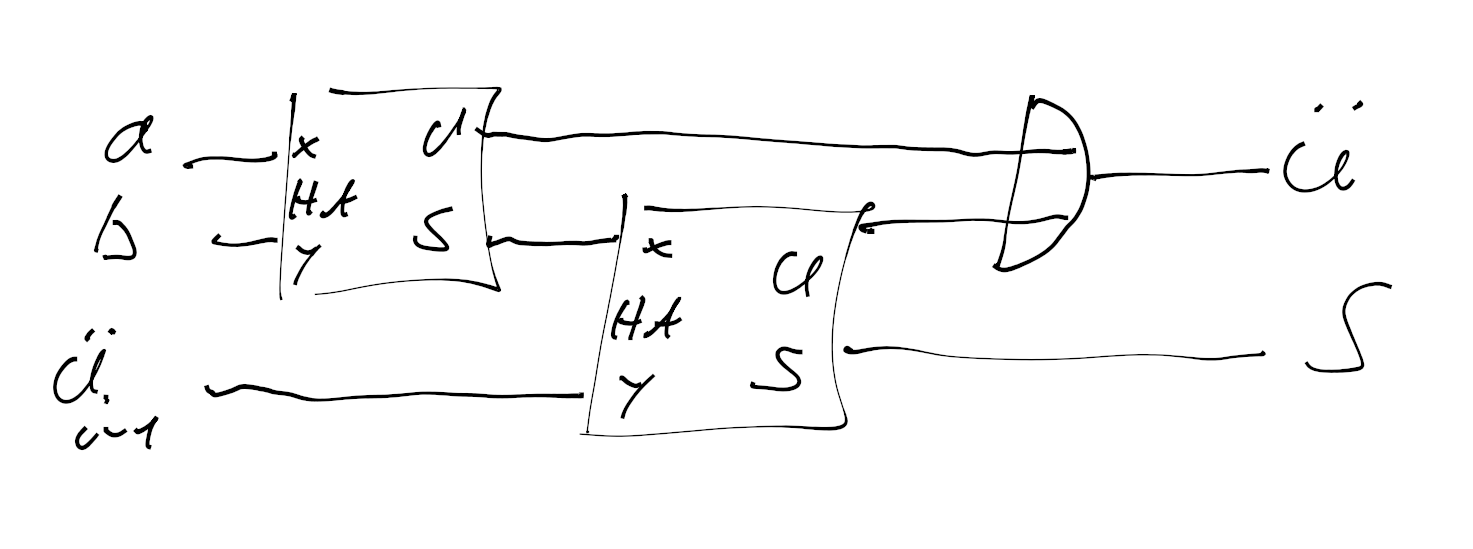
\includegraphics[width=1\textwidth]{volladdierer.png}
		\captionof{figure}{Volladdierer aus zwei Halbaddierern.}
		\label{fig:volladdierer}
	\end{Figure}

	\subsection*{Q}
	In Abb. \ref{fig:sadd} ist ein serielles Addierwerk dargestellt.
	\begin{Figure}
		\centering
		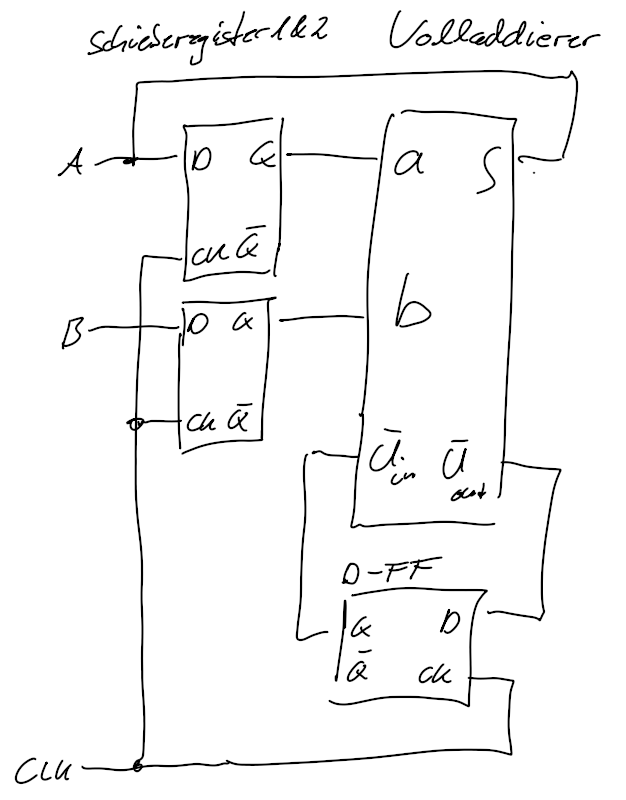
\includegraphics[width=0.8\textwidth]{serielles_addierwerk.png}
		\captionof{figure}{Serielles Addierwerk}
		\label{fig:sadd}
	\end{Figure}
	\section{Auswertung}
        \subsection{e) \& f)}
        Mit dem seriell oder parallel ladbaren n-Bit Schieberegister lässt sich eine n-Bit Zahl speichern und wieder ausgeben.
        Die Schaltskizzen sind in den Voraufgaben zu finden.
        Im Versuch wurde erfolgreich ein serielles 4-Bit und parallels 3-Bit Schieberegister aufgebaut.
        Das 3-Bit Schieberegister wurde auch als Ringschieberegister aufgebaut, indem der letzte Ausgang wieder an den Eingang angeschlossen wird, was es möglich macht, die Zahl \glqq im Kreis\grqq{} durch das Register zu schieben.
        Verschiedene Zahlen konnten gespeichert und ausgelesen werden; die Schaltung (oder Speichern und Auslesen der Bits) funktioniert nach dem FIFO Prinzip.

        \subsection{g)}
        Mit den beiden Halbaddierern kann ein Volladdierer gebaut werden, welcher, durch Verwendung zweier serieller 3-Bit Ringschieberegistern zu einem Addierwerk verbaut werden kann.
        Dieses wurde bereits in den Voraufgaben besprochen.
        Dieses Addierwerk kann zwei 3-Bit Zahlen addieren, allerdings nur bis maximal \texttt{111} darstellen.
        Das Limit ist also die Größe des Ringschiebers.
        \par Eine Zahl kann durch umlegen eines Schalters in einen Ringschieber eingelesen werden.
        Indem man die Ringschieber taktet \glqq rutscht\grqq{} der Bit von der dritten Stelle $\left(3_2=4_{10}\right)$ zur zweiten $\left(2_2=2_{10}\right)$ und zur ersten Stelle $\left(1_2=1_{10}\right)$.
        Durch weitere drei Takte können diese beiden Zahlen addiert werden.
        Das Addieren funktioniert so, dass immer jeweils ein Bit aus den Ringschiebern mit dem Volladdierer addiert werden und der Übertrag wieder in den Eingang des Volladdierers eingeführt wird.
        Das Ergebnis wird im ersten Ringschieber angezeigt (die eingegebenen Zahlen gehen dabei verloren).
        Einige Beispiele sind
        \begin{align} 
                001+000&=001&011+001&=100&100+011&=111
        .\end{align} 
        
	\section{Fazit}
        In diesem Versuch wurde die Übertragungskennlinie eines Invertierers (aufgebaut aus CMOS) gemessen.
        Mit Hilfe dieser CMOS wurde ein NAND Gatter gebaut, für welches wieder die Übertragungskennlinie gemessen wurde.
        Beide Kennlinien haben den theoretischen Erwartungen entsprochen.
        \par Danach wurde Schritt für Schritt ein serielles 3-Bit Addierwerk aufgebaut.
        Angefangen mit einem XOR-Gatter aus NAND-Gattern zu einem Halbaddierer und dann einem Volladdierer, indem ein zweiter Halbaddierer gebaut wurde und die Überträge entsprechend zurückgeführt wurden.
        Mit einem seriellen 3-Bit Ringschieber konnten dann zwei verschiedene Zahlen eingelesen werden und durch drei mal takten (da es sich hier um 3-Bit Zahlen handelt) des Volladdierers addiert werden.
        Das Ergebnis wurde in einem Ringschieber gespeichert und konnte durch Abgreifen der Ausgänge angezeigt werden.
\end{multicols}
\end{document}
